\documentclass[11t]{article}
\usepackage[margin=1.0in]{geometry}
\usepackage{graphicx}
\usepackage{hyperref}
\usepackage{cite}
\usepackage{fancybox,ascmac}
\usepackage{amsmath,amssymb}
\usepackage{type1cm}
\usepackage{amsthm}
\usepackage{nccmath}
\usepackage{enumitem}
\usepackage{hyperref}
\usepackage{cite}

\title{\large{Multi-period Stochastic Optimization Models for Dynamic Asset Allocation}}
\author{
    Masaya Tsukamoto\thanks{Master's student of Quantitative Finance \& Risk Management} \\
    \texttt{masayats@umich.edu}
}

\date{}

\begin{document}
\maketitle

\begin{abstract}

Optimization of multi-period asset allocation strategy has been an important problem for long-term institutional investors and has been tackled in the finance field. The hybrid model that combines Monte-Carlo simulation and the scenario-tree model is proposed by Hibiki \cite{hybrid}. Two different types of approaches, fixed-unit strategy and fixed-proportion strategy, can be considered as the hybrid model. The fixed-unit strategy version is a linear programming problem, which is much easier to solve. However, practitioners prefer to manage their portfolio by the proportion of each risky asset in the total asset.  The fixed-proportion strategy problem is exactly what investors want to solve, but it is a non-convex problem. To handle this situation, the iterative algorithm is also proposed where we can finally solve the fixed-proportion strategy problem by solving the fixed-unit strategy several times. In this report, The hybrid model and the iterative algorithm are implemented by Python. It is confirmed that the optimal multi-period strategy is indeed obtained in reasonable time even if ten thousands of Monte-Carlo paths are applied. This model is very valuable from the practical perspective because it is compatible with any type of scenario-generating models.

\end{abstract}

\section{Introduction}
Optimization of multi-period asset allocation strategy has been an important problem for long-term institutional investors such as insurance companies and pension funds.

To find the optimal strategy under uncertainty of the future, the scenario-tree model is a popular approach \cite{tree},
where future scenarios of the financial market and their associated probability are explicitly set via tree-structure. 
We can consider portfolio rebalancing strategies depending on the future situations, but the computational cost grows exponentially as the number of rebalancing strategy branchpoints (or nodes) of the scenario tree.
As a result, the number of rebalancing points is usually not large enough to describe the detail of future uncertainty.

Using Monte-Carlo simulation for future asset returns is another approach \cite{sim}. Even though it can cover future uncertainty in detail and the simulating model is flexible, 
we cannot apply different rebalancing strategies depending on different future states. In other words, we have to fix only one rebalancing strategy which should be applied in any simulated future paths.

The hybrid model \cite{hybrid} is proposed to take advantage and overcome the shortcomings of the above two approaches.
First, Monte-Carlo simulation is conducted. Then, rebalancing strategy branchpoints are created by bundling the simulated paths.
Once the simulated paths and the strategy branchpoints are determined, maximization of the investor's utility function will be conducted to obtain the optimal investment strategies.
See Fig \ref{str} for a simple description of the structures of these three models.

\begin{figure}[htbp]
\centering
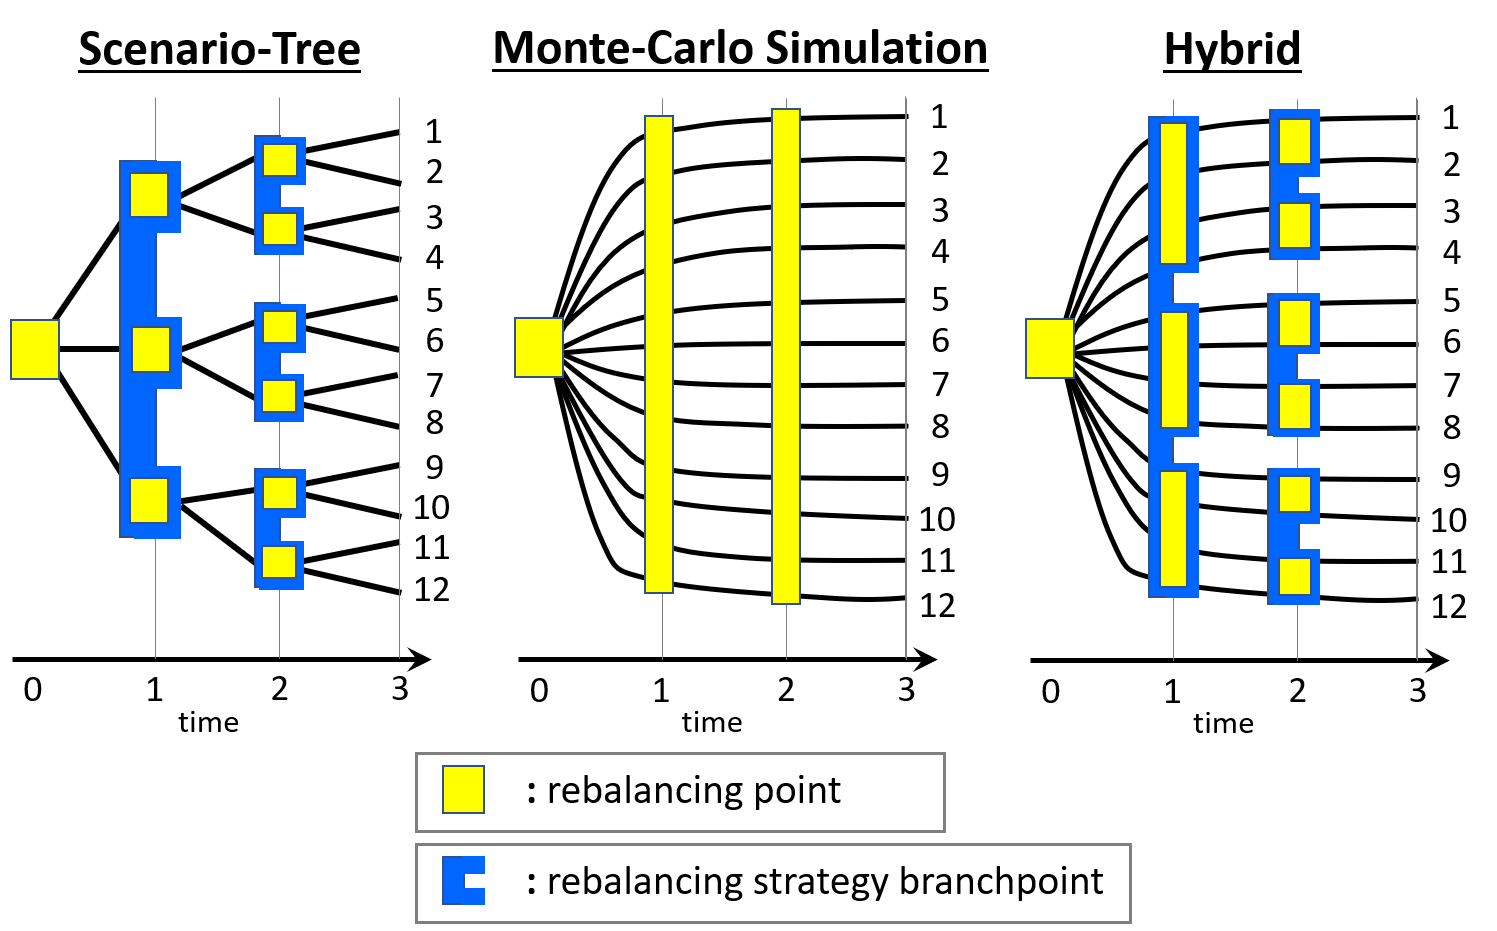
\includegraphics[width=0.6\textwidth]{structure.png}
\caption{Structure of the three approach}
\label{str}
\end{figure}

\section{Optimization Problem}
\subsection{Principles}
There are risky assets, such as stocks, available in the financial market. Investors can decide how much they invest in each risky asset. They can also invest in cash (or ``bank account"), which can be considered as a risk-free asset. The expected returns of the risky assets are typically higher than that of cash (risk-free interest rate). However, future returns of the risky assets will fluctuate stochastically and cannot be perfectly predicted. Then, investors will be faced with the optimization problem how to allocate their total wealth to risky assets and cash.

Typical investors prefer higher expected returns and smaller risk (uncertainty). Therefore it is natural that the objective function is usually defined in the form of the expected wealth at the end of the investment period minus some risk measure.

\subsection{Notation}
{\bf (1) Sets}
\begin{description}
\setlength{\leftskip}{0.3in}
  \item[$S_t$] : set of fixed-decision nodes (rebalancing strategy branchpoints) at time $t$ $(s \in S_t)$.
  \item[$V_t^s$] : set of Monte-Carlo simulation paths passing any fixed-decision node $s$ at time $t$ $(i \in V_t^s)$. 
\end{description}
{\bf (2) Parameters}
\begin{description}
\setlength{\leftskip}{0.3in}
  \item[$I$] : number of Monte-Carlo simulation paths.
  \item[$n$] : number of risky asset.
  \item[$T$] : number of investment time periods.
  \item[$\rho_{j0}$] : price of risky asset $j$ at time 0 $(j=1,...,n)$.
  \item[$\rho_{jt}^{(i)}$] : price of risky asset $j$ of path $i$ at time $t$ $(j=1,...,n; t=1,...,T; i=1,...,I)$.
  \item[$r_0$] : risk-free interest rate from time 0 to 1.
  \item[$r_{t}^{(i)}$] : risk-free interest rate of path $i$, from time $t$ to $t+1$ $(t=1,...,T-1; i=1,...,I)$.
  \item[$W_0$] : initial total wealth.
  \item[$W_G$] : target terminal total wealth.
  \item[$\gamma$] : risk aversion coefficient.
\end{description}
{\bf (3) Decision variables}
\begin{description}
\setlength{\leftskip}{0.3in}
  \item[$z_{j0}$] : base investment unit for risky asset $j$ at time $0$ $(j = 1,...,n)$.
  \item[$z_{jt}^{s}$] : base investment unit for risky asset $j$ at time $t$ and node $s$ $(j = 1,...,n; t=1,...T; s \in S_t)$.
  \item[$v_{0}$] : cash at time 0.
  \item[$v_{t}^{(i)}$] : cash of path $i$ at time $t$ $(t=1,...T-1; i=1,...,I)$.
  \item[$q^{(i)}$] : shortfall below target terminal total wealth of path $i$ $(i=1,...,I)$.
\end{description}

\subsection{Formulation}
Assume the rebalansing points are given to focus on the optimization part. As the hybrid model, there can be two different types of problems:
 Fixed-unit strategy and Fixed-proportion strategy. \vspace{3mm} \\
%\min_{x \in \mathbb{R}^n} 
{\bf \underline{Formulation}}
\begin{flalign}
\max_{z_{j0}, z_{jt}^s, v_0, v_t^{(i)}, q^{(i)}}  &  \hspace{4mm} \frac{1}{I} \sum_{i=1}^{I} W_T^{(i)} - \gamma \left( \frac{1}{I} \sum_{i=1}^{I} q^{(i)} \right)&  \label{obj}
\end{flalign}
{\rm subject to:}
\begin{fleqn}
\begin{gather}
\hspace{10mm} W_0 = \sum_{j=1}^{n} \rho_{j0} z_{j0} + v_0  \label{eq1}  \\
\hspace{10mm} \sum_{j=1}^{n} \rho_{j1}^{(i)} z_{j0} + (1+r_0) v_0 = \sum_{j=1}^{n} \rho_{j1}^{(i)} z_{j1} + v_1   \hspace{0.2in} (s \in S_1; i \in V_1^s)  \label{eq2} \\
\hspace{10mm} \sum_{j=1}^{n} \rho_{jt}^{(i)} h^{(i)} ( z^{s'}_{j,t-1} ) + (1+r^{(i)}_{t-1}) v^{(i)}_{t-1} 
			=  \sum_{j=1}^{n} \rho_{jt}^{(i)} h^{(i)} (z^{s}_{jt}) + v^{(i)}_{t}  \hspace{0.2in} (t=2,...,T-1 ; s \in S_t; i \in V_t^s) \label{eq3} \\
\hspace{10mm}  \sum_{j=1}^{n} \rho_{jT}^{(i)} z^{s'}_{j,T-1} + (1+r^{(i)}_{T-1}) v^{(i)}_{T-1} = W_T^{(i)} \hspace{0.2in} (s' \in S_{T-1}; i \in V_{T-1}^{s'}) \label{eq4} \\
\hspace{10mm} W_T^{(i)} + q^{(i)} \geq W_G  \hspace{0.4in}  (i=1,...,I) \label{q1} \\
\hspace{10mm} z_{j0} \geq 0   \hspace{1.0in}  (j=1,...,n) \label{z1} \\
\hspace{10mm} z^s_{jt} \geq 0  \hspace{1.0in}  (j=1,...,n; t=1,...,T-1; s \in S_{t}) \label{z2} \\
\hspace{10mm} v_{0} \geq 0  \label{v1} \\
\hspace{10mm} v_t^{(i)} \geq 0 \hspace{1.0in}  ( t=1,...,T-1; i=1,...,I)   \label{v2} \\
\hspace{10mm} q^{(i)} \geq 0 \hspace{1.0in}   (i=1,...,I)    \label{q2}
\end{gather}
\end{fleqn}
{\bf \underline{Fixed-unit strategy}}
\begin{fleqn}
\begin{gather}
\hspace{5mm} h^{(i)} ( z^{s}_{jt} ) = z^{s}_{jt}   \label{fix_unit}
\end{gather}
\end{fleqn}
Investment units have the same value for all paths passing any rebalancing point for risky assets. Cash has the different value for any paths. \vspace{3mm} \\
{\bf \underline{Fixed-proportion strategy}}
\begin{fleqn}
\begin{gather}
\hspace{5mm} h^{(i)} ( z^{s}_{jt} ) = \left( \frac{ W_t^{(i)}}{ \rho_{jt}^{(i)} } \right) z^{s}_{jt}   \label{fix_prop}
\end{gather}
\end{fleqn}
$W_t^{(i)}$ is a total wealth of path $i$ at time $t$. Investment proportions have the same value for all paths passing any rebalancing point for any assets including cash.


\subsection{Interpretation of the formulation}
The objective function (\ref{obj}), or the investor's utility function, has the form of the expected terminal wealth minus a risk measure. The risk measure used here is the first-order lower partial moment (${\rm LPM}_1$). 
Combined with the inequality constraints (\ref{q1}) and (\ref{q2}), ${\rm LPM}_1$ can be written as below. ${\rm LPM}_1$ works as a penalty when the terminal wealth goes below the target.
\begin{equation*}
{\rm LPM}_1 =  \frac{1}{I} \sum_{i=1}^{I} q^{(i)}  =  \frac{1}{I} \sum_{i=1}^{I} \max \left\{ W_G - W_T^{(i)}, 0 \right\}
\end{equation*}
Because $W_G$ is a given parameter and $W_T^{(i)}$ is determined by the other variables than $q^{(i)}$, which are $ \left( z_{j0},  z^s_{jt}, v_{0}, v_t^{(i)} \right)$, at least one equality of the two inequalities (\ref{q1}) and (\ref{q2}) must hold for each $i$ in the optimal point to make the objective function large as possible.
These $q^{(i)}$ are introduced as slack variables to decompose the $\max \left\{*, 0 \right\}$ function in ${\rm LPM}_1$ and make this optimization problem a linear programming.

The equality constraints (\ref{eq1}) and (\ref{eq4}) correspond to the definition of the total wealth. The equality constraints (\ref{eq2}) and (\ref{eq3}) mean that rebalancing the portfolio does not change the total wealth. In other words, any new money will not be added to this investment project and any money will not be subtracted from this project during the investment period (from $t=0$ to $t=T$). This is called the ``self-financing" condition in the financial field.

The inequality constraints (\ref{z1}) and (\ref{z2}) mean that investors cannot hold the negative amount of risky assets. In financial terminology, ``short-selling" is not allowed. Similarly, the inequality constraints (\ref{v1}) and (\ref{v2}) mean that investors cannot hold the negative amount of cash.

The function $h^{(i)} ( z^{s}_{jt} )$ is introduced to describe both formulations of the fixed-unit and fixed-proportion strategies in a single way. 
 $h^{(i)} ( z^{s}_{jt} )$ itself means the unit and we can simply set  $h^{(i)} ( z^{s}_{jt} ) =  z^{s}_{jt} $ (\ref{fix_unit}) in the fixed-unit strategy.
In the fixed-proportion strategy, by regarding  $h^{(i)} ( z^{s}_{jt} ) = \left( \frac{ W_t^{(i)}}{ \rho_{jt}^{(i)} } \right) z^{s}_{jt}$  (\ref{fix_prop}) as the unit, 
then the decision variable $z^{s}_{jt} =  \left( \frac{ \rho_{jt}^{(i)} }{ W_t^{(i)}} \right)  h^{(i)} ( z^{s}_{jt} )$ turns to represent the proportion.

\subsection{Iterative algorithm}
The fixed-proportion strategy is exactly what investors are interested in. However, this is a non-convex problem because $W^{(i)*}_t$ is a function of decision variables. On the other hand, even though the fixed-unit strategy is inconvenient in practice, it is a linear optimization problem easier to solve. 
To take advantage of both benefits of these strategies, the iterative algorithm is proposed. \vspace{3mm} \\

{\bf \underline{Iterative algorithm}}
\begin{enumerate}
\item Solve the fixed-unit strategy problem and calculate the wealth of path$i$ at time $t$, $W_{t(0)}^{{(i)*}}$, which is used as an initial value.
\item For the $k$-th iteration, set up $ h^{(i)} ( z^{s}_{jt} ) = \left( \frac{ W_{t(k-1)}^{(i)*}}{ \rho_{jt}^{(i)} } \right) z^{s}_{jt} $ as the investment unit function, and solve the problem.
\item If a change of the objective fuction value is small enough, stop. Otherwise, set $k \leftarrow k + 1$ and return to 2. 
\end{enumerate}

\section{Implementation and Result}
The author of the original paper used a commercial optimization software to solve the problem and didn't publish his code. In this report, the algorithm is implemented using Python and PuLP package because they are available for any researchers and practitioners.
\subsection{Basic Parameters}

\begin{itemize}
  \item \# of risky assets: $n$=2,  \hspace{1em} \# of paths: $I$ = 10000,  \hspace{1em} \# of time periods: $T$ = 6.
  \item $r_0$ = $r_{t}^{(i)}$ = 0.01. All interest rates are constant, not depending on $t$ and $i$. 
  \item Risk aversion coefficient: $\gamma$ = 20.0
  \item Initial wealth: $W_0 = 100$, \hspace{1em} Target wealth: $W_G = 100$
\end{itemize}

\subsection{Input scenarios}
The biggest advantage of the hybrid model from the practitioners' viewpoint is the point that simulated paths of asset returns can be regarded as just input parameters, 
which means the hybrid model is compatible with any types of Monte-Carlo simulation model about the financial market. 

In this section, the returns of the risky assets are simply generated by the normal distribution. This scenarios of the returns are just input data and are not critical in a demonstration of the proposed model and algorithm. The normal distribution parameters for the returns are described as below.
\begin{itemize}
  \item Mean of the returns of Risky Asset 1 and Risky Asset 2 are 0.03 and 0.04, respectively.
  \item Standard deviation of the returns of Risky Asset 1 and Risky Asset 2 are 0.1 and 0.2, respectively.
  \item Correlation of the returns of Risky Asset 1 and Risky Asset 2 is $-0.5$.
\end{itemize}

\subsection{Strategy branchpoint}
To simplify the situation, only one strategy branchpoint is introduced at time $t=3$. If path $i$ satisfies the following condition:
\begin{equation*}
\frac{1}{2} \sum_{j=1}^{2} \frac{1}{3} \sum_{t=1}^{3} \left[ \textrm{return from time } t-1 \textrm{ to time } t, \textrm{ of risky asset } j, \textrm{ of path } i  \right] > \frac{1}{2} (0.03 + 004)
\end{equation*}
then path $i$ is classified as Branch A, otherwise Branch B. The idea is simple: Branch A means ``better than average so far" and Branch B means ``worse than average so far". The structure of this model is describe in Fig \ref{one_branch}.
\begin{figure}[htbp]
\centering
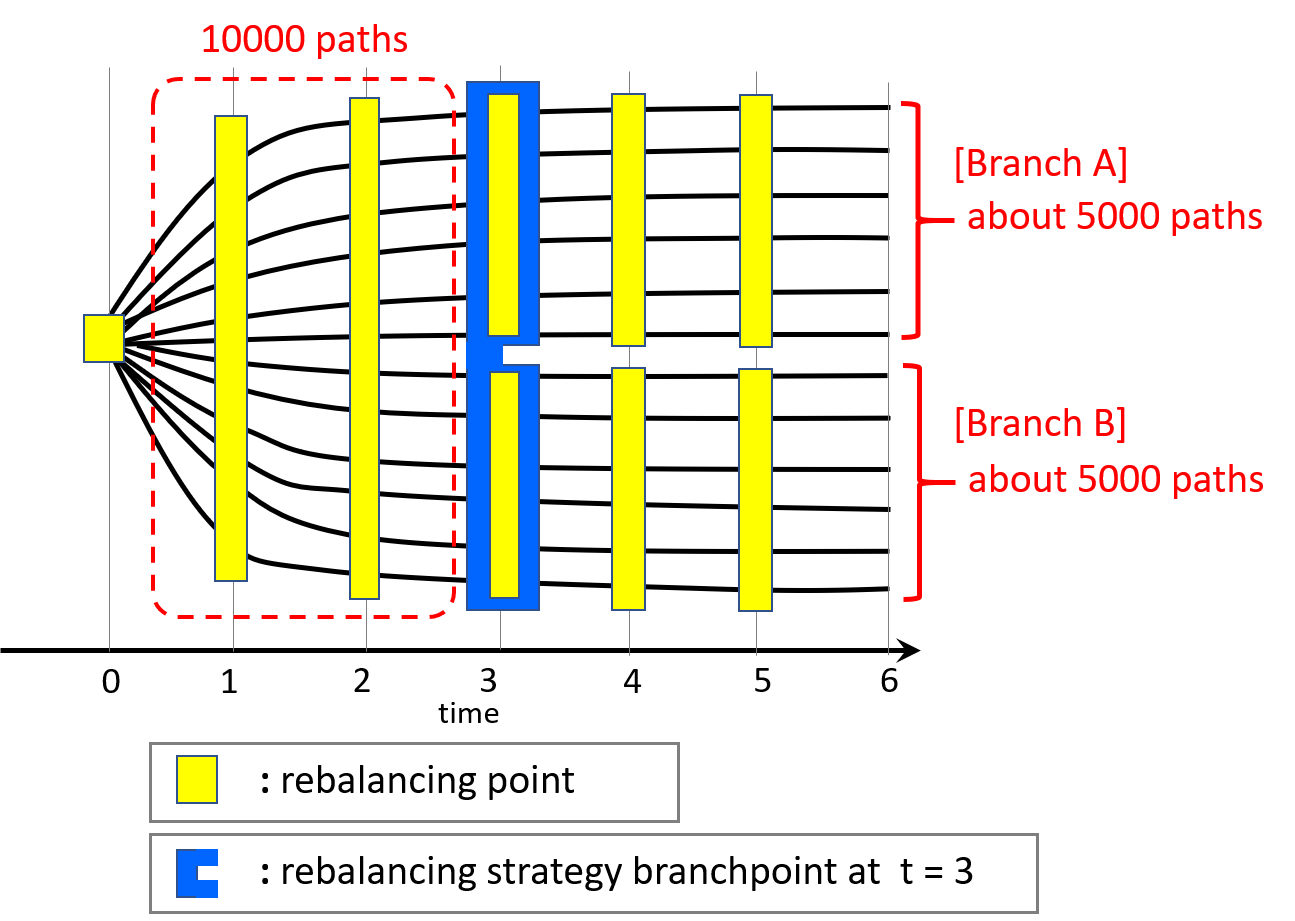
\includegraphics[width=0.6\textwidth]{one_branch.png}
\caption{Structure of the implemented model}
\label{one_branch}
\end{figure}

\subsection{Result: Optimal Proportion}
The optimal proportion based on the fixed-proportion problem is successfully obtained. The computational time is about 919 seconds with the ordinary laptop (OS: 64-bit Windows 10, CPU: Intel Core i5-8250U@1.60GHz, RAM: 8.00GB), which is very comfortably fast. The results are described in Fig \ref{branch_A} and Fig \ref{branch_B}.

\begin{figure}[htbp]
\centering
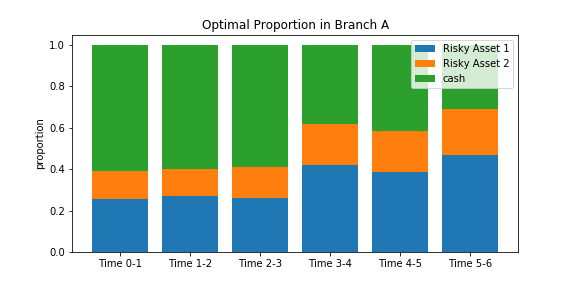
\includegraphics[width=0.7\textwidth]{optimal_proportion_A.png}
\caption{Optimal proportion of Branch A}
\label{branch_A}
\end{figure}
\begin{figure}[htbp]
\centering
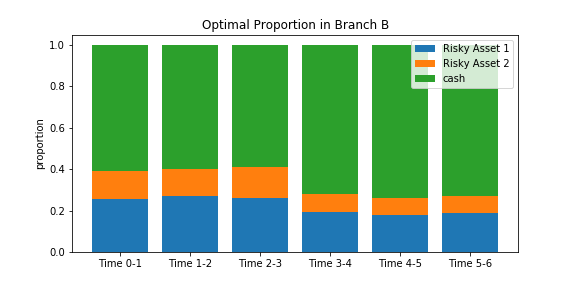
\includegraphics[width=0.7\textwidth]{optimal_proportion_B.png}
\caption{Optimal proportion of Branch B}
\label{branch_B}
\end{figure}

Overall, Risky Asset 1 is preferred to Risky Asset 2. This is because the standard deviation of returns of Risky Asset 1 is much smaller than that of Risky Asset 2 even though the expected return of Risky Asset 1 is slightly smaller.  These two portfolio transitions inevitably have the same proportions until the branchpoint $t=3$ but fork into different strategies from the branchpoint. It is very reasonable that Branch A has larger proportions of risky assets because in Branch A the investors should have extra wealth to invest aggressively, but in Branch B the investors should be less rich and more careful about their potential loss, then they couldn't take a risk. 

\subsection{Percentiles of total wealth}
To examine the status of the total wealth, percentiles (99\%, 90\%, 50\%, 10\%, 1\%) over the paths are plotted in Fig \ref{per}.
The left corresponds to percentiles over the whole 10000 paths.
The middle is percentiles over paths that belong to Branch A after $t$ = 3, which contain 5061 paths.
Similarly, the right is over 4939 paths that belong to Branch B.

\begin{figure}[htbp]
\begin{center}
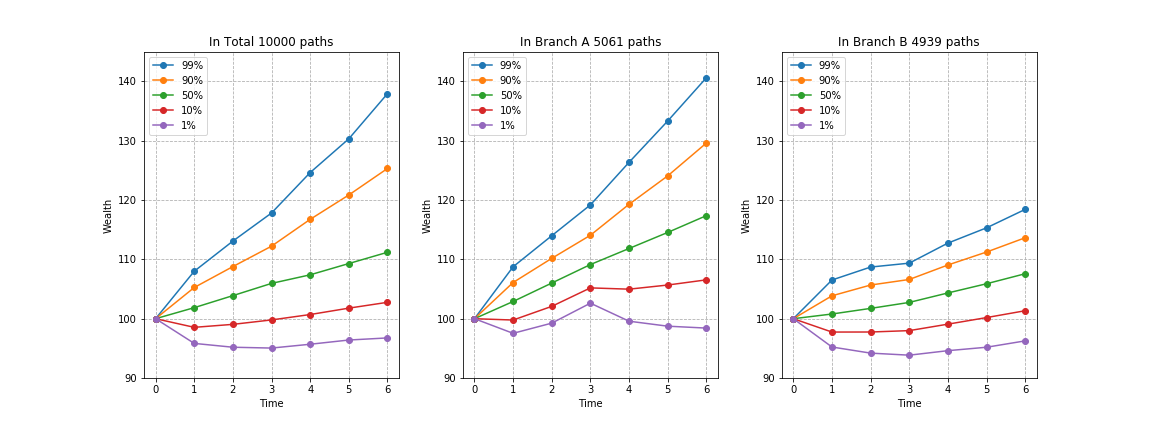
\includegraphics[width=1.0\linewidth,clip]{wealth_percentile.png}
\caption{Percentiles of total wealth at each time}
\label{per}
\end{center}
\end{figure}

Because paths in Branch A and B are picked up based on the status until $t=3$,
it is natural by definition that the wealth of Branch A is biased higher and that of Branch B is lower.
We can see that the difference between 99\%-ile and 1\%-ile is expanding after $t$ = 3 in Branch A more than in Branch B.
This is consistent with the fact that the optimal portfolio in Branch A is holding more risky assets than in Branch B.
Because of the reduced proportions of the risky assets in Branch B, the investor can keep the 10\% and 1\% graphs flat or even increasing, preventing a further loss.

\subsection{Convergence of the iterative algorithm}
The values of objective function during the iterative algorithm is described in Fig \ref{conv}. The convergence criteria used here is that changes in proportions of any risky asset at any time is smaller than $10^{-6}$. Then, the algorithm converges after 7 iterations. According to Fig \ref{conv}, the algorithm actually almost converges after 3 or 4 iterations. By definition of the iterative algorithm, the value of the objective function after 1 iteration is the optimal objective function value of the fixed-unit strategy problem. Therefore, it implies that the fixed-proportion strategy can attain a higher value of the investor's utility function than the fixed-unit strategy.
\begin{figure}[htbp]
\centering
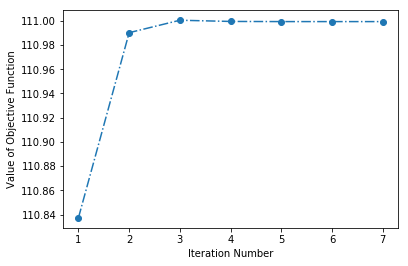
\includegraphics[width=0.6\textwidth]{conv.png}
\caption{Values of objective function}
\label{conv}
\end{figure}

\section{Conclusion}
The proposed model and algorithm is confirmed to actually work in a reasonable time, even if it is implemented by Python. The optimal fixed-proportion strategy can be obtained and makes sense. The iterative algorithm looks stable and only several iterations are required for convergence. 

From the viewpoint of practitioners, the biggest advantage of the hybrid model is the fact that paths of asset returns can be regarded as just input parameters, which means it is compatible with any types of simulating models about the financial market. Many financial institutions have their own stochastic scenario generators and want to optimize their portfolio based on their scenarios. Therefore, it is valuable especially for practitioners to make the algorithm openly available.

\section{Practical use}
After investors obtains the optimal portfolio strategy as described in Fig \ref{branch_A} and  Fig \ref{branch_B}, they will allocate their asset at $t = 0$, following the first [Time 0-1] proportion. After that, they typically rerun the simulation and optimization regularly, e.g., once a year, using up-to-date information. And then, again they will follow the first [Time 0-1] proportion obtained from the newest optimization. 

The natural question is: why do they have to consider long-term future scenarios even though they actually use only the first, short-term proportion?
The reason is there are significantly non-zero autocorrelations in time-series of asset returns 
and the investors have to care about their long-term solvency taking into account the autocorrelations.
A bond is a simple example.
A whole return during the 10-year investment period of the 10-year bonds is determined at the moment of purchase (if the issuer's default risk is ignored). 
However, in the short term, the price of the 10-year bonds may fluctuate.
If the price significantly dropped in a year, it will recover during the remaining 9 years. 
Therefore investors, especially those who place importance on the long-term solvency such as life insurance companies and pension fund, 
should determine their asset allocation strategy based on the long‐term viewpoint.


\bibliography{reference}{}
\bibliographystyle{unsrt}

\end{document}